\documentclass[aspectratio=169]{beamer}
\input{../header}

\title{Stochastic Process}
\author{Md. Aminul Islam Shazid}
\date{}

\usepackage{booktabs}

\begin{document}
    {
		\setbeamertemplate{footline}{}
		\addtocounter{framenumber}{-2}
 
		\begin{frame}
			\titlepage
		\end{frame}
 
		\begin{frame}{Outline}
            \vfill
			\tableofcontents[subsectionstyle=hide]
            \vfill
		\end{frame}
	}
 
    \section{Stochastic Process}
 
    \begin{frame}{Stochastic Process}
        \begin{itemize}
            \item A stochastic process $\{X(t): t \in T\}$ is a family of random variables indexed by a parameter $t$, which runs over an index set $T$.
            \item The parameter $t$ usually denotes time.
            \item For any specific time $t$, $X(t)$ is a random variable.
            \item The index set $T$ is called the parameter set.
            \item If $T$ is countable, $\{X(t)\}$ is a discrete time stochastic process. If $T$ is an interval, finite or infinite, $\{X(t)\}$ is a continuous time stochastic process.
            \item The set of possible values of $X(t)$ at any time $t$ is called the state space, $S$.
        \end{itemize}
    \end{frame}
 
    \begin{frame}{Example}
        A business office has five telephone lines and any number of these lines may be in use at any time. The telephone lines are observed at regular intervals of 2 minutes.
 
        $X$: Number of lines in use in every 2 minutes.
 
        For $T = 0, 1, 2, 3, \ldots$,
        \[
        X(t): \{X(0), X(1), X(2), \ldots\} \quad \text{e.g. } X(t): \{3, 2, 5, 0, 1, 0, 3, \ldots\}
        \]
 
        Here, $\{X(t): t \in T\}$ is a stochastic process with parameter space $T = \{0, 1, 2, 3, \ldots\}$ and state space $S = \{X: 0, 1, 2, 3, 4, 5\}$.
    \end{frame}
 
    \begin{frame}{Graphical Example}
        An observation of this process might look like below.
 
        \begin{figure}
            \centering
            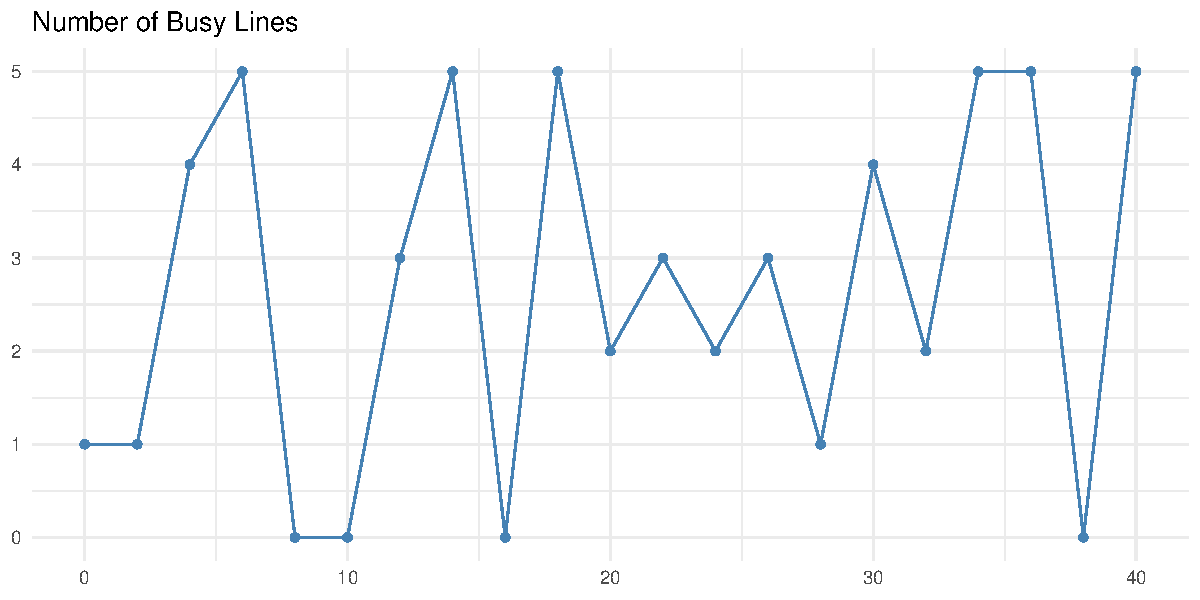
\includegraphics[width=0.85\textwidth]{plots/busy-lines.pdf}
        \end{figure}
    \end{frame}
 
    \begin{frame}{Examples of some stochastic processes}
        \textbf{1. Random walk model:} Let $X_t$ be a random variable that can be any of the two states [up ($+1$) or down ($-1$)] at time $t$.
 
        \begin{table}
            \centering
            \begin{tabular}{lcc}
                \toprule
                $X_t$ & $+1$ & $-1$ \\
                \midrule
                probability & $p$ & $1-p$ \\
                \bottomrule
            \end{tabular}
        \end{table}
 
        Then, the process $R_t = R_{t-1} + X_t$ is called a random walk model.
 
        \textbf{2. Counting process:} A stochastic process $\{N(t); t > 0\}$ is a counting process if $N(t)$ represents the total number of events that have occurred in time $t$.
 
        \textbf{3. Birth \& death process:} A stochastic process $\{N(t); t \geq 0\}$ with states $\{n = 0, 1, 2, \ldots\}$ for which transition from state $n$ may go only to either of the states $(n-1)$ or $(n+1)$ is a birth and death process.
    \end{frame}
 
    \begin{frame}{Autocorrelation or Serial Correlation}
    \begin{itemize}
        \item In statistics, the autocorrelation of a random process describes the correlation between values of the process at different times, as a function of the two times or of the time lag.
        \item Let $X$ be some repeatable process, and $i$ be some point in time after the start of that process. Then $X_i$ is the value (or realization) produced by a given run of the process at time $i$.
        \item The autocorrelation between times $s$ and $t$ is defined as $R(s,t) = \mathrm{Corr}(X_t, X_s)$, the correlation coefficient between $X_t$ and $X_s$.
        \end{itemize}
    \end{frame}
 
 
    \section{Markov Process}
 
 
    \begin{frame}
    \frametitle{Markov Process}
        \begin{itemize}
            \item Consider a set of points $(t_0, t_1, \ldots, t_n, t)$, where $t_0 < t_1 < \cdots < t_n < t$ and $t, t_i \in T$ ($i = 0, 1, 2, \ldots, n$); $T$ is a parameter space of the process $\{X(t)\}$.
            \item The dependence exhibited by the process $\{X(t): t \in T\}$ is called Markovian dependence if the conditional distribution of $X(t_{n+1})$ for given values of $X(t_0), X(t_1), X(t_2), \ldots, X(t_n)$ depends only on $X(t_n)$, which is the most recent known value of the process, i.e., if
            \begin{align*}
                &\Pr[X(t_{n+1}) = x \mid X(t_n) = x_n, X(t_{n-1}) = x_{n-1}, \ldots, X(t_0) = x_0] \\
                &= \Pr[X(t) = x \mid X(t_n) = x_n]
            \end{align*}
        \end{itemize}
        The stochastic process exhibiting this property (Markov property) is called a Markov process.
    \end{frame}
 
 
    \begin{frame}{Types of Markov Process}
        \begin{table}
            \centering
            \resizebox{\textwidth}{!}{%
            \begin{tabular}{lcc}
                \toprule
                & \multicolumn{2}{c}{State space} \\
                Parameter space & Discrete & Continuous \\
                \midrule
                Discrete & Markov chain & Discrete parameter, continuous MP \\
                Continuous & Continuous parameter, discrete MC & Continuous parameter, continuous MP \\
                \bottomrule
            \end{tabular}%
            }
        \end{table}
 
        \textbf{Notations:}
        \[
        p_i = \text{Probability that the process is in state } i \text{ at a given time}
        \]
        \begin{align*}
            p_{ij}^{(n)} &= n\text{-step transition probability of state } j \text{ from state } i \\
            &= \Pr[\text{process moves from } i \text{ to } j \text{ in } n \text{ steps}]
        \end{align*}
    \end{frame}
 
 
    \begin{frame}{Transition Probability Matrix (TPM)}
        A matrix containing probabilities of transition from one state to another. If there are $k$ finite states of a Markov process, i.e. $S = \{1, 2, \ldots, k\}$, the one-step TPM is
        \[
            P = \begin{pmatrix} p_{11} & p_{12} & \cdots & p_{1k} \\ p_{21} & p_{22} & \cdots & p_{2k} \\ \vdots & \vdots & \ddots & \vdots \\ p_{k1} & p_{k2} & \cdots & p_{kk} \end{pmatrix}
        \]
            such that (i) $p_{ij} \geq 0, \; \forall i, j \in S$; (ii) $\sum_j p_{ij} = 1$ (row total 1).
    \end{frame}
 
    \begin{frame}{Markov Process: Example 1}
        \begin{columns}
            \begin{column}{0.45\textwidth}
                $X$ = living status. State space $S = \{1, 2, 3\}$; where $1 =$ healthy, \\
                $2 =$ sick, $3 =$ dead.
                \[
                    P = \begin{pmatrix} p_{11} & p_{12} & p_{13} \\ p_{21} & p_{22} & p_{23} \\ p_{31} & p_{32} & p_{33} \end{pmatrix}
                \]
                Here, $p_{31} = p_{32} = 0$; $p_{33} = 1$, and all other probabilites are above zero and below 1 (non-zero, not one).
            \end{column}
            \begin{column}{0.45\textwidth}
                \begin{figure}
                \centering
                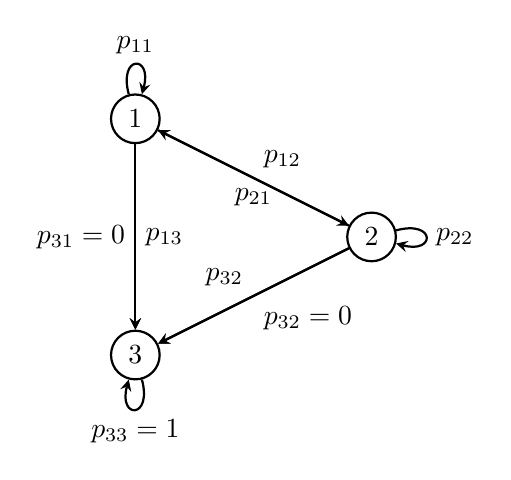
\begin{tikzpicture}[node distance=2.5cm, >=stealth, thick]
                    \node[circle, draw] (1) at (0, 1.5) {1};
                    \node[circle, draw] (2) at (3, 0) {2};
                    \node[circle, draw] (3) at (0, -1.5) {3};
                    \draw[->] (1) to[loop above] node[above] {$p_{11}$} (1);
                    \draw[->] (2) to[loop right] node[right] {$p_{22}$} (2);

                    \draw[->] (3) to[loop below] node[below] {$p_{33} = 1$} (3);

                    \draw[->] (1) -- node[above right] {$p_{12}$} (2);
                    \draw[->] (2) -- node[below] {$p_{21}$} (1);
                    \draw[->] (1) -- node[right] {$p_{13}$} (3);
                    \draw[->] (2) -- node[above left] {$p_{32}$} (3);
                    
                    \draw[->] (1) -- node[left] {$p_{31} = 0$} (3);
                    \draw[->] (2) -- node[below right] {$p_{32} = 0$} (3);
                \end{tikzpicture}
                \end{figure}
            \end{column}
        \end{columns}
    \end{frame}
 
 
    \begin{frame}{Stationary Markov Chains}
        \textbf{Time-homogeneous Markov chains} (or stationary Markov chains) are processes where
        \[
            \Pr[X_{t+1} = x \mid X_t = y] = \Pr[X_t = x \mid X_{t-1} = y]
        \]
        for all $t$. The probability of the transition is independent of $t$.
    \end{frame}
 
 
    \begin{frame}{Classification of states}
        \begin{itemize}
            \item \textbf{Accessible state:} A state $j$ is said to be accessible from a state $i$ (written $i \to j$) if a system started in state $i$ has a non-zero probability ($p_{ij} > 0$) of transitioning into state $j$ at some point.
            \item \textbf{Communicating states:} A state $i$ is said to communicate with state $j$ (written $i \leftrightarrow j$) if both $i \to j$ and $j \to i$. Here, $p_{ij} > 0$ and $p_{ji} > 0$.
            \item \textbf{Absorbing state:} A state $i$ is called absorbing if it is impossible to leave this state. Therefore, state $i$ is absorbing if and only if $p_{ii} = 1$ and $p_{ij} = 0$ for $i \neq j$.
        \end{itemize}
    \end{frame}
 
    \begin{frame}{Classification of states (cont.)}
        \begin{itemize}
            \item \textbf{Transient state \& recurrent state:} A state $i$ is said to be transient if, given that we start in state $i$, there is a non-zero probability that we will never return to $i$. State $i$ is recurrent (or persistent) if it is not transient. Recurrent states are guaranteed (with probability 1) to have a finite hitting time.
            \item \textbf{Periodic state \& aperiodic state:} A state $i$ has period $k$ if any return to state $i$ must occur in multiples of $k$ time steps. A state is aperiodic if returns to state $i$ can occur at irregular times ($k=1$).
        \end{itemize}
    \end{frame}
 
    \begin{frame}{Multi-step transitions}
        \begin{itemize}
            \item The $n$-step TPM is obtained by multiplying the one-step TPM by itself $n$ times: $P^{(n)} = P^n$. Its $(i,j)$th entry, $p_{ij}^{(n)}$, is the probability of moving from state $i$ to state $j$ in $n$ steps.
            \item If $A = (p_1, p_2, \ldots, p_k)$ is the probability vector (distribution over states) at time 0, then the distribution after $n$ steps is
            \[
            A^{(n)} = A \cdot P^n
            \]
            \item This can be computed either as $A^{(n)} = A^{(n-1)} \cdot P$ (applying $P$ one step at a time) or directly as $A \cdot P^{(n)}$ once $P^{(n)}$ is known — both give the same result.
        \end{itemize}
    \end{frame}
 
    \begin{frame}{Example 2}
        There are two telephone lines in an office and any number of these lines may be in use at any given time. Telephone lines are observed at regular intervals of 2 minutes. The initial probability vector of the states is
        \[
            A = (0.3, 0.5, 0.2)
        \]
        and the one-step transition probability matrix is
        \[
            P = \begin{pmatrix} 0.2 & 0.6 & 0.2 \\ 0.3 & 0.5 & 0.2 \\ 0.1 & 0.4 & 0.5 \end{pmatrix}
        \]
        Assuming a time-homogeneous Markov chain $X_t$, determine the probabilities that no line, 1 line, and 2 lines are being used at (i) $t=1$, (ii) $t=2$ (starting time $t=0$). Also find $\Pr[X_0 = 1, X_1 = 0, X_2 = 2]$.
 
        Let $0$: no line in use, $1$: 1 line in use, $2$: 2 lines in use, so $S = \{0, 1, 2\}$.
    \end{frame}
 
    \begin{frame}{Example --- solution}
        \textbf{For $t=1$:}
        \[
            A^{(1)} = AP = (0.3, 0.5, 0.2) \begin{pmatrix} 0.2 & 0.6 & 0.2 \\ 0.3 & 0.5 & 0.2 \\ 0.1 & 0.4 & 0.5 \end{pmatrix} = (0.23, 0.51, 0.26)
        \]
 
        \textbf{For $t=2$:}
        \[
            A^{(2)} = A^{(1)} P = (0.23, 0.51, 0.26) \begin{pmatrix} 0.2 & 0.6 & 0.2 \\ 0.3 & 0.5 & 0.2 \\ 0.1 & 0.4 & 0.5 \end{pmatrix} = (0.225, 0.497, 0.278)
        \]
    \end{frame}
 
 
    \begin{frame}{Example --- solution}
        Find $\Pr[X_0 = 1, X_1 = 0, X_2 = 2]$.
        \begin{align*}
            \Pr[X_0 = 1, X_1 = 0, X_2 = 2] &= \Pr[X_2 = 2 \mid X_1 = 0] \, \Pr[X_1 = 0 \mid X_0 = 1] \, \Pr[X_0 = 1] \\
            &= p_{02} \, p_{10} \, p_1
        \end{align*}
        using the Markov property, $\Pr[X_2 = 2 \mid X_1 = 0, X_0 = 1] = \Pr[X_2 = 2 \mid X_1 = 0]$.
 
        So,
        \[
            \Pr[X_0 = 1, X_1 = 0, X_2 = 2] = p_1 \, p_{10} \, p_{02} = 0.5 \times 0.3 \times 0.2 = 0.03
        \]
    \end{frame}
 
    \begin{frame}{Steady State Probabilities}
        If, for an irreducible Markov chain (only one class, so all states communicate), all states are aperiodic and positive recurrent (returns in finite time), the distribution $A^{(n)} = A \cdot P^n$ converges as $n \to \infty$, and the limiting distribution is independent of the initial probabilities $A$:
        \[
            \lim_{n \to \infty} p_{ij}^{(n)} = \lim_{n \to \infty} a_j^{(n)} = p_j
        \]
        These are called steady state probabilities, and satisfy
        \[
            p_j > 0, \qquad \sum_{j=0}^{m} p_j = 1, \qquad p_j = \sum_{i=0}^{m} p_i \, p_{ij}, \quad j = 0, 1, \ldots, m
        \]
        Since there are $m+2$ equations but only $m+1$ unknowns, one equation is redundant — use $m$ of the $m+1$ equations above together with $\sum_j p_j = 1$.
    \end{frame}
 
    \begin{frame}{Example 3}
        Find the steady state probabilities for the Markov chain in Example 2.
 
        At steady state,
        \[
            (p_0, p_1, p_2) = (p_0, p_1, p_2) \begin{pmatrix} 0.2 & 0.6 & 0.2 \\ 0.3 & 0.5 & 0.2 \\ 0.1 & 0.4 & 0.5 \end{pmatrix}
        \]
        which gives the system
        \[
            \begin{aligned}
                -0.8 p_0 + 0.3 p_1 + 0.1 p_2 &= 0 \\
                0.6 p_0 - 0.5 p_1 + 0.4 p_2 &= 0 \\
                p_0 + p_1 + p_2 &= 1
            \end{aligned}
        \]
        (the third original balance equation is redundant given $\sum p_j = 1$).
    \end{frame}
 
    \begin{frame}{Example --- solution}
        Solving the system by elimination gives
        \[
            p_0 = \frac{17}{77}, \qquad p_1 = \frac{38}{77}, \qquad p_2 = \frac{22}{77}
        \]
 
        These are the long-run (steady state) probabilities that 0, 1, and 2 telephone lines are in use, respectively, regardless of the initial distribution $A$.
    \end{frame}
 
\end{document}
